% Version 3.1 December 2024
% Springer Nature LaTeX Template for Masters-Paper-
\documentclass[pdflatex,sn-mathphys-num]{sn-jnl}% APA Reference Style
\usepackage{comment}
\usepackage[T1]{fontenc}%
\usepackage{graphicx}%
\usepackage{multirow}%
\usepackage{amsmath,amssymb,amsfonts}%
\usepackage{amsthm}%
\usepackage{mathrsfs}%
\usepackage[title]{appendix}%
\usepackage{xcolor}%
\usepackage{textcomp}%
\usepackage{manyfoot}%
\usepackage{booktabs}%
\usepackage{algorithm}%
\usepackage{algorithmicx}%
\usepackage{algpseudocode}%
\usepackage{listings}%
\usepackage{tikz}%
\usetikzlibrary{arrows.meta,positioning,shapes.geometric}%

\newcommand{\juhoansi}{\mbox{Ju\textbar{}'hoansi}}%

\theoremstyle{thmstyleone}%
\newtheorem{theorem}{Theorem}%
\newtheorem{proposition}[theorem]{Proposition}%

\theoremstyle{thmstyletwo}%
\newtheorem{example}{Example}%
\newtheorem{remark}{Remark}%

\theoremstyle{thmstylethree}%
\newtheorem{definition}{Definition}%

\raggedbottom

\begin{document}

\title[Computational Narrative Modeling for Indigenous Knowledge Preservation]{\juhoansi{} Narrative Agentic Generator (\texttt{jnang}): Ontologically Grounded Agentic Narrative Generation and Cultural Adaptation for Indigenous African Oral Traditions}

%%=============================================================%%
%% Authors and Affiliations
%%=============================================================%%
\author*[1]{\fnm{Lemuel} \sur{Mayinoti}}\email{lemuel.Mayinoti@nust.na}
\author[1]{\fnm{Naftali} \sur{Indongo}}\email{nindongo@nust.na}
\author[1]{\fnm{Heike} \sur{Winschiers-Theophilus}}\email{hwinschiers@nust.na}

\affil*[1]{\orgdiv{Department of Software Engineering}, \orgname{Namibia University of Science and Technology}, \orgaddress{\street{13 Jackson Kaujeua Street}, \city{Windhoek}, \country{Namibia}}}
%%==================================%%
%% Abstract                         %%
%%==================================%%

\abstract{Large Language Models (LLMs) can generate fluent stories, but their training data provide limited representation of many indigenous African oral traditions. As a result, generated narratives may reproduce culturally inappropriate structures even when they contain appropriate cultural vocabulary. This work investigates whether combining culturally grounded narrative structures with knowledge-graph retrieval and multi-agent generation can improve the cultural authenticity of generated \juhoansi{} folktales. We introduce the \textit{\juhoansi{} Narrative Agentic Generator (\texttt{jnang})}, which represents narrative knowledge using an RDF ontology and Neo4j knowledge graph and uses specialised agents for generation, structural classification, and evaluation. The system draws on established folkloristic approaches, including Dundes' motifemes and Camp/Bush spatial structure, to guide narrative generation beyond surface-level retrieval. In a pilot evaluation of 16 generated narratives, \texttt{jnang} outperformed a naive baseline on cultural authenticity across all 8 tested themes under independent judging (sign test, $p \approx 0.004$). The baseline also produced European cultural tropes in 2 of 8 stories, while \texttt{jnang} produced none. Importantly, this pilot evaluation relied entirely on LLM-based judges and deterministic keyword checks; no \juhoansi{} community members participated in evaluating the generated stories. The results are further limited by the small sample size and incomplete coverage of the source corpus. These findings suggest that culturally structured retrieval and multi-agent generation are a promising direction for computational approaches to indigenous narrative generation, but meaningful claims about cultural authenticity require validation with \juhoansi{} speakers and communities.}

\keywords{Computational Folkloristics, Indigenous Knowledge Preservation, Large Language Models, Multi-Agent Systems, Knowledge Graphs, \juhoansi{}, Narrative Generation}

\maketitle

\section{Introduction}\label{sec:intro}

Large Language Models (LLMs) now generate fluent narrative prose across creative and academic writing tasks \cite{naveed2023comprehensive,Khurana2023}. That fluency comes from training corpora dominated by high-resource Indo-European languages, so indigenous African oral traditions such as \juhoansi{} folklore receive almost no representation \cite{Adelani2022,Lo}. Prompted to generate a \juhoansi{} narrative, an LLM does not fail outright; it produces a fluent story that smuggles in the wrong culture.

\textit{Monarchs} replace \textit{elders}, \textit{gold and coin} replace \textit{honey and meat}, and a hoarding protagonist meets \textit{execution} rather than \textit{communal reconciliation}. Each substitution erases the egalitarian, non-hoarding ethic and the Camp/Bush spatial structure that organize authentic \juhoansi{} storytelling, leaving a Western tale dressed in \juhoansi{} vocabulary.

Agentic systems narrow this gap by giving LLMs access to real \juhoansi{} folktales absent from their training data, typically through Retrieval-Augmented Generation (RAG) \cite{lewis2020retrieval} that retrieves story excerpts by semantic similarity. Semantic retrieval surfaces passages with the right objects and settings, but it does not preserve the sequence of motifemes, the taboo-violation-consequence chain, or the movement between Camp and Bush that give a \juhoansi{} narrative its structure. A retrieved excerpt can be lexically authentic while the story built around it stays structurally Western.

We address this with Graph-RAG \cite{edge2024graphrag}: retrieval grounded in narrative structure rather than text similarity. This paper introduces \texttt{jnang}, the \juhoansi{} Narrative Agentic Generator, which pairs a Neo4j Knowledge Graph encoding Alan Dundes' 8 motifemes and Lévi-Straussian Camp/Bush spatial dynamics with a Generator Agent that conditions \texttt{gpt-4o-mini} on Cypher-retrieved subgraphs. The graph gives the Generator Agent each excerpt's structural role in the narrative, not just its surface content, so the resulting \juhoansi{} narratives stay structurally coherent as well as culturally grounded.

\subsection{Background}
The \juhoansi{} San community of Donkerbos, in Namibia's Omaheke region, historically subsisted through foraging across more than 100 plant and 40 animal species, and since the 1970s has shifted toward a mixed economy of foraging, wage labor, and craft sales while retaining this ecological knowledge \cite{wiessner2014}. Campfire storytelling remains central to \juhoansi{} social life, transmitting elder wisdom, maintaining social harmony, and framing puberty rites and healing dances \cite{wiessner2014,keeney2013reentry}. This work extends an ongoing collaborative research initiative under the UNESCO Chair in Digital Technology Design with Indigenous People at the Namibia University of Science and Technology, which co-designs technologies with the Donkerbos \juhoansi{} community to support their social, educational, and economic resilience \cite{Kays2023}.

\subsection{Objectives}
The main objective of this work is to model, engineer, and evaluate \texttt{jnang}, an ontologically grounded multi-agent narrative generator that produces culturally authentic, structurally sound \juhoansi{} stories from existing San oral traditions. This decomposes into three sub-objectives:

\begin{enumerate}
    \item \textbf{Ontological Formalization}: Create an ontology  of existing Ju|hoansi narratives from Alan dundes  motifeme morphology and turn it into a  Neo4j Knowledge Graph.
    \\
    \item \textbf{Agentic Steering}: Develop a 3-agent LangGraph pipeline (Generator, Classifier, Evaluator), with this paper centered on the \textit{Generator Agent}, which constrains LLM (\texttt{gpt-4o-mini}) output through ontology- and graph-grounded context to eliminate Western narrative tropes.
    \\
    \item \textbf{Evaluation \& Benchmarking}: Benchmark AI-generated narratives against human-curated \juhoansi{} folktales on cultural authenticity, motifeme coherence, non-hoarding adherence, and click-consonant orthographic precision.
\end{enumerate}



%
% \subsection{Contributions}
% \begin{enumerate}
%     \item \textbf{Indigenous Narrative Ontology}: A formal RDF Turtle narrative ontology (\texttt{folktales\_ontology.ttl}) mapping Alan Dundes' 8 canonical motifemes \cite{dundes1964morphology}, Proppian moves, and Lévi-Straussian spatial axes (Camp vs. Bush) to \juhoansi{} socio-ecological dynamics.
%     \item \textbf{Graph-Grounded Generator Agent}: A 3-agent LangGraph pipeline (Generator, Classifier, Evaluator) supporting end-to-end generation and grading; this paper centers on the \textit{Generator Agent}, contextualized via Cypher queries over a Neo4j Knowledge Graph to synthesize motifeme- and spatially-constrained \juhoansi{} narratives.
%     \item \textbf{Machine Translation & Adaptation Framework}: A Pre-Translation Oicotype Adaptation mechanism enabling standard MT architectures to perform cultural and structural alignment before target token generation in low-resource African languages.
%     \item \textbf{Empirical Evaluation}: Quantitative benchmarking against human-curated \juhoansi{} folktales, showing cultural authenticity, structural brevity, and elimination of Eurocentric tropes.
% \end{enumerate}
% %
\section{Related Work}\label{sec:related}

\subsection{Computational Folkloristics \& Story Generation}
Automated Story Generation (ASG) moved from rule-based planners such as TALESPIN and FABULIST to transformer-based neural generators trained on large text corpora \cite{naveed2023comprehensive}. Computational folklorists parsed folk narrative structure using Proppian functions and the Aarne-Thompson-Uther (ATU) tale-type index \cite{propp1928morphology}. Finlayson's \texttt{ProppLearner} corpus and structure-learning algorithms extended this by annotating and automatically inferring Proppian functions from Russian folktale text \cite{finlayson2012learning,finlayson2017propplearner}, but this line of work targets and validates against Propp's Indo-European functions specifically, leaving non-Proppian oral traditions unaddressed. Modern LLMs produce fluent prose against these same Western-derived benchmarks, but fluency is judged against Indo-European narrative arcs, leaving open whether the same models can represent story structures the benchmarks never encode.

\subsection{African NLP \& Indigenous Knowledge Preservation}

African languages remain under-represented in NLP research due to data scarcity and the limited availability of digital infrastructure for low-resource machine translation and language modelling \cite{Adelani2022,Lo}. \juhoansi{} has a limited corpus of annotated oral narratives available for computational use. At present, efforts are underway to crowdsource and develop such a corpus. \cite{indongo2026designing} demonstrate that introducing digital technologies into \juhoansi{} communities requires participatory co-design and cultural alignment with the community itself, rather than focusing solely on linguistic coverage. This requirement is equally important when developing systems for generating \juhoansi{} narratives, where cultural accuracy and community perspectives must be considered alongside linguistic and computational performance \cite{indongo2025mirror}.


\subsection{Formalist Paradigms: Propp, Dundes, and Lévi-Strauss}

Propp identified 31 functions that describe the structure of Russian fairy tales \cite{propp1928morphology}. These functions encode a linear quest arc driven by an individual hero who departs home, acquires magical helpers, defeats a villain, and receives a reward of monarchy, marriage, or wealth ($W^*$). The model assumes static character spheres (Hero, Villain, Donor, Princess) and reaches closure through punishment of the antagonist.

Dundes \cite{dundes1964morphology} argued that Propp's functions are specific to Indo-European tale traditions and do not generalize to oral traditions with different social structures. Working with Native American and African corpora, Dundes identified smaller structural units called \textit{motifemes}: recurring narrative positions (Lack, Interdiction, Violation, Consequence, Mediation, Lack Liquidated, Departure, Return) that combine in short, often symmetrical chains rather than Propp's extended 31-step sequences. Critically, Dundes' motifemes do not presuppose individual heroism, monarchical authority, or punitive antagonist resolution, making them structurally compatible with oral traditions grounded in communal ethics and egalitarian social organization. No prior computational system has used Dundes' motifeme framework as a generative constraint; existing computational narrative work, including Finlayson's \texttt{ProppLearner} \cite{finlayson2012learning,finlayson2017propplearner}, targets and validates against Proppian functions exclusively.

Lévi-Strauss \cite{levistrauss1955structural} offered a complementary perspective, analyzing myths through opposing binary categories (nature/culture, raw/cooked, human/supernatural) rather than sequential functions. For \juhoansi{} narratives, the distinction between the human \textbf{Camp} (social order, kinship obligations, communal fire) and the supernatural \textbf{Bush} (ancestral spirits $g//awasi$, ecological danger, metamorphosis) provides a spatial and ontological axis that organizes narrative movement. However, Lévi-Strauss' structural analysis describes the logic of mythical thought rather than providing a generative grammar for sequencing narrative events.

We adopt Dundes' motifemes as the primary generative constraint for three reasons: (1) they were developed for non-European oral traditions and avoid encoding Indo-European cultural assumptions; (2) their compact, episodic chains match the brevity and symmetry of \juhoansi{} storytelling as documented by Biesele \cite{biesele2006ju}; and (3) they provide sequenceable narrative positions suitable for computational implementation. We supplement Dundes with Lévi-Strauss' Camp/Bush spatial axis, which provides the cultural geography that motifeme chains alone do not encode.

\subsection{Knowledge Graphs \& Multi-Agent Frameworks}

Knowledge graphs provide a structured way of representing entities and their relationships. Semantic Web standards such as RDF and OWL support the representation of this knowledge in a machine-readable form, with Turtle providing a compact serialization format \cite{w3c2014rdfconcepts,w3c2014turtle,w3c2012owl2}. RAG allows language models to incorporate information retrieved from external knowledge sources \cite{lewis2020retrieval}. GraphRAG extends this approach by retrieving connected information from knowledge graphs, helping models maintain relationships between multiple pieces of information \cite{edge2024graphrag}. Graph databases such as Neo4j provide infrastructure for storing and querying such structured knowledge \cite{clemedtson2025graphraft}. Multi-agent frameworks such as LangGraph \cite{langchain2024langgraph}, AutoGen \cite{wu2023autogen}, and MetaGPT \cite{hong2023metagpt} enable language models to work through specialised agents with different roles and responsibilities \cite{wu2023autogen,hong2023metagpt}. These approaches provide more structured workflows than relying on a single language-model interaction and have increasingly been explored for complex generation and reasoning tasks.
\medskip


\section{Method}\label{sec:theory}

The methodology followed a sequential process from source analysis to narrative generation. First, \juhoansi{} folktales were analysed using Dundes' motifemes and Proppian narrative functions. The resulting structures were formalised in an RDF/OWL ontology and represented in a Neo4j knowledge graph. This structured knowledge, together with retrieved textual material and lexical constraints, was then used by the LangGraph multi-agent pipeline to generate and classify narratives. Finally, the generated narratives were evaluated for structural and cultural appropriateness.

% \juhoansi{} oral tradition relies on four cultural mechanics:

% \begin{table}[h]
% \caption{Western formalist tropes compared to \juhoansi{} oral epistemologies.}\label{tab:comparison}
% \begin{tabular}{@{}lll@{}}
% \toprule
% Dimension & Western Formalism (Propp) & \juhoansi{} Formalism (\texttt{jnang}) \\
% \midrule
% Role Model & Static (Hero, Villain, Donor) & Fluid (Trickster = Troublemaker + Helper) \\
% Primary Reward ($W^*$) & Monarchy, Gold, Marriage & Communal Food Sharing ($zo$ honey, meat, water) \\
% Spatial Dynamic & Linear Quest Arc & Spatial Axis (Camp $\leftrightarrow$ Bush Transformation) \\
% Structural Length & Long (31 functions) & Compact Motifemes (3--6 Dundes units) \\
% Antagonist Resolution & Execution / Punishment & Social Reconciliation / Communal Alignment \\
% Ecological Oicotypes & Magic Sword, Castle, Crown & Gemsbok Horn, Digging Stick, $n\textbar{}um$ Energy \\
% \bottomrule
% \end{tabular}
% \end{table}

% \subsection{Cultural and Theoretical Foundation}

% \texttt{jnang} adapts Alan Dundes' eight nuclear motifemes \cite{dundes1964morphology} to \juhoansi{} narratives: \textbf{Lack} (scarcity of honey, $zo$, water, or meat), \textbf{Interdiction} (a taboo stated by an elder, $!ga$ or $!o$), \textbf{Violation} (breaking the interdiction), \textbf{Consequence} (ecological or spiritual effects), \textbf{Mediation} (intervention by an ancestral spirit, $g//awasi$, or animal helper), \textbf{Lack Liquidated} (communal sharing and restoration), \textbf{Departure} (transition from Camp to Bush), and \textbf{Return} (return from Bush to Camp).





% \section{System Architecture}\label{sec:architecture}

% The \texttt{jnang} architecture links three layers: the Semantic Ontology Layer, the Knowledge Graph Context Builder, and the LangGraph Multi-Agent Pipeline.

% \begin{figure}[h]
% \centering
% \begin{tikzpicture}[
%     node distance=1.1cm,
%     layer/.style={rectangle, draw, rounded corners, minimum width=8cm, minimum height=1.1cm, align=center, fill=gray!8},
%     arr/.style={-{Latex[length=2.5mm]}, thick}
% ]
% \node[layer] (ont) {Semantic Ontology Layer\\\texttt{folktales\_ontology.ttl} (RDF/OWL)};
% \node[layer, below=of ont] (kg) {Knowledge Graph Layer\\Neo4j + \texttt{context\_builder.py}};
% \node[layer, below=of kg] (agents) {LangGraph Multi-Agent Pipeline\\Generator $\rightarrow$ Classifier $\rightarrow$ Grader};

% \draw[arr] (ont) -- (kg) node[midway, right, font=\footnotesize] {\texttt{import\_rdf.py}};
% \draw[arr] (kg) -- (agents) node[midway, right, font=\footnotesize] {Cypher subgraph retrieval};
% \end{tikzpicture}
% \caption{Three-layer \texttt{jnang} architecture. An RDF/OWL ontology is ingested into a Neo4j knowledge graph, which supplies theme-matched subgraphs to the LangGraph multi-agent pipeline at generation time.}
% \label{fig:architecture}
% \end{figure}

% \subsection{Corpus & Structural Decomposition}
% We draw source material from \textit{\juhoansi{} Folktales: Transcriptions and English Translations} \cite{biesele2009folktales}, a community-authored literacy primer of 14 transcribed \juhoansi{} folktales with interlinear \juhoansi{}-English translations, compiled by Megan Biesele together with named \juhoansi{} transcribers and translators. A companion lexicon (\texttt{ju\_dictionary.xls}) supplies 4{,}737 term-level entries mapping \juhoansi{} vocabulary to English senses and parts of speech, used to constrain the Generator Agent's vocabulary and verify orthography.

% Of these 14 stories, we formalized four --- \textit{The Moon Dies and Lives Again}, \textit{The Honey and the Flies}, \textit{A Woman First Found Fire}, and \textit{The Elephant First Found Water} --- into the seed RDF knowledge graph described below. For each story, an LLM first proposed a candidate segmentation into Dundes motifemes, Proppian narrative-function moves, character roles, and Camp/Bush spatial tags; a human reviewer then corrected this segmentation against the source transcription before encoding it as RDF triples. We use LLM-assisted rather than fully automatic annotation deliberately: an unsupervised LLM is exactly the failure mode this paper documents (Section~\ref{sec:intro}), so every motifeme and move in the ground-truth ontology is human-verified rather than model-asserted. The remaining ten stories serve as unstructured RAG excerpts, retrievable by the Generator Agent for lexical and thematic grounding but not yet decomposed into explicit motifeme chains.

% \subsection{RDF Narrative Ontology & Neo4j Knowledge Graph}
% We defined an RDF Turtle schema (\texttt{folktales\_ontology.ttl}) using OWL classes:
% \begin{lstlisting}[language=TeX]
% propp:Character a owl:Class .
% propp:NarrativeFunction a owl:Class .
% propp:MagicalAgent rdfs:subClassOf propp:Object .
% propp:ProppianRole a owl:Class .
% \end{lstlisting}

% \texttt{import\_rdf.py} ingests RDF triples into Neo4j, creating graph relationships (\texttt{:PERFORMS\_FUNCTION}, \texttt{:HAS\_ROLE}, \texttt{:LACKS}, \texttt{:FOLLOWS}). At runtime, \texttt{context\_builder.py} executes Cypher queries matching the narrative theme to load subgraphs into the Generator Agent's context window.

% \begin{figure}[h]
% \centering
% 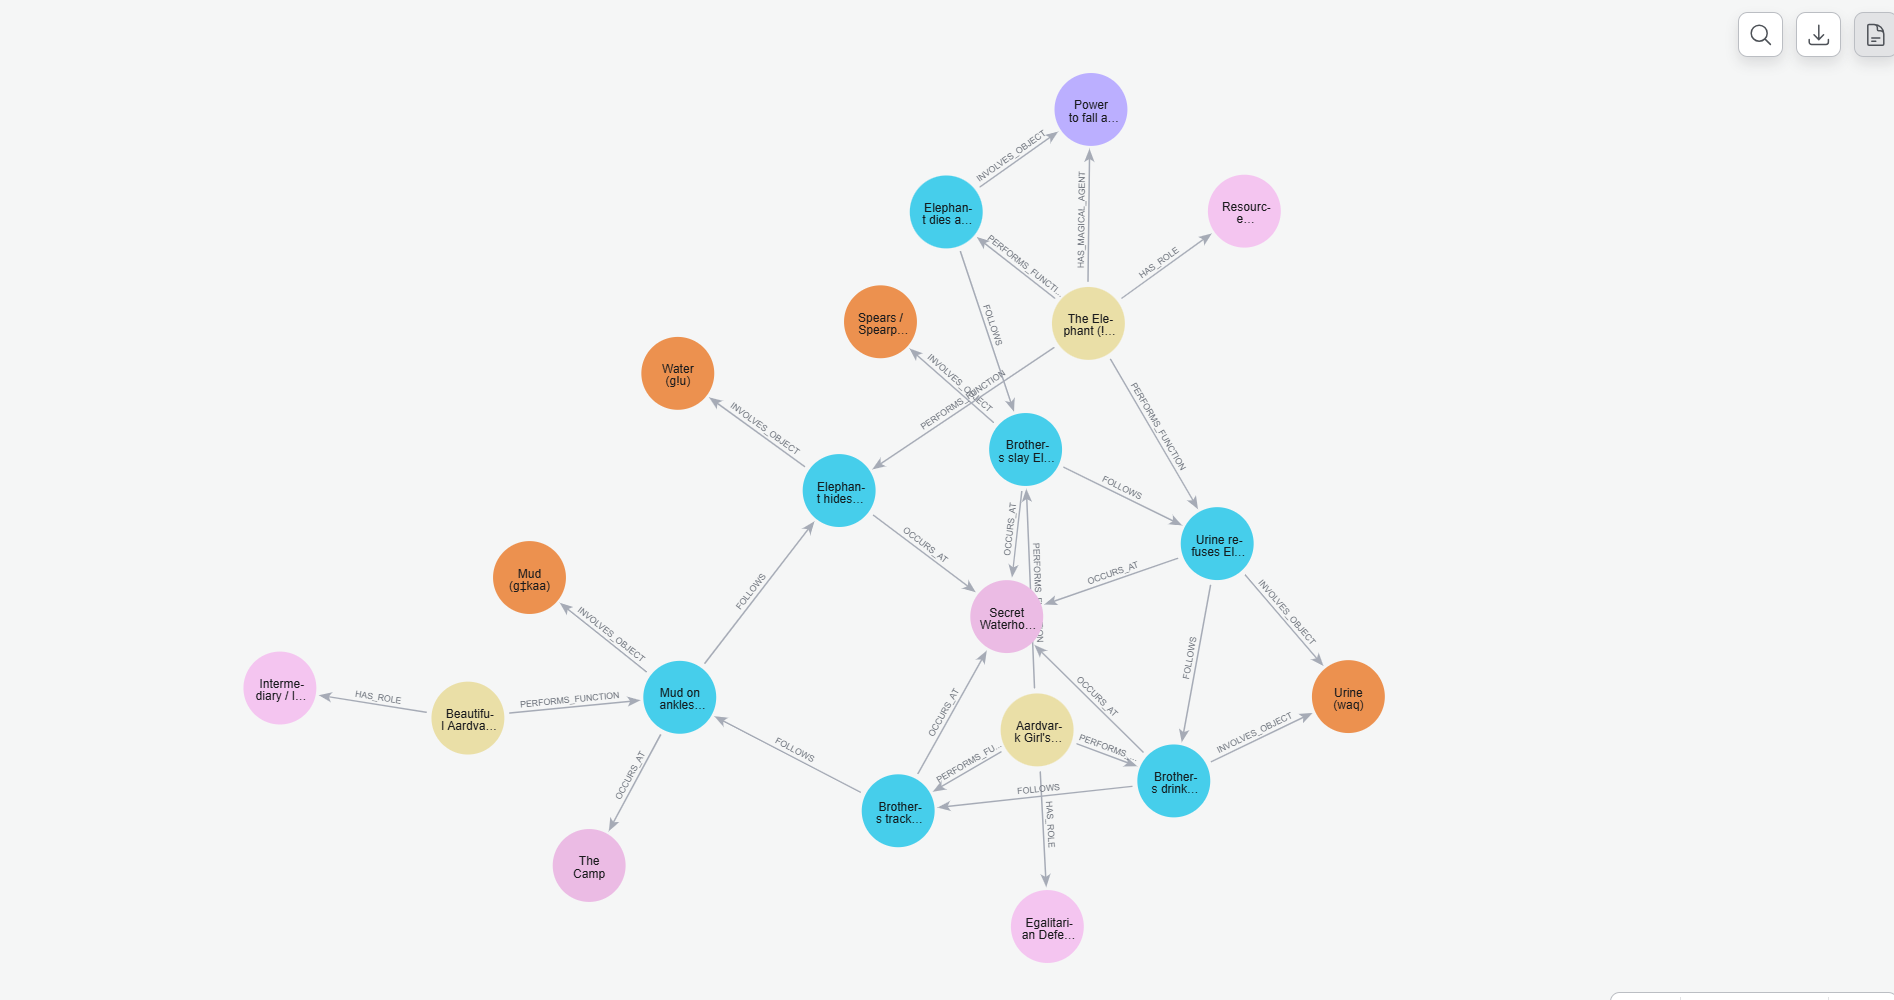
\includegraphics[width=\textwidth,trim=10 10 10 10,clip]{figures/kg-2hop-query.png}
% \caption{Neo4j 2-hop neighborhood query around a story's narrative functions. Typed relationships --- \texttt{PERFORMS\_FUNCTION}, \texttt{HAS\_ROLE}, \texttt{FOLLOWS}, \texttt{INVOLVES\_OBJECT}, \texttt{OCCURS\_AT}, \texttt{HAS\_MAGICAL\_AGENT} --- connect characters, narrative functions, objects, roles, and locations for the \textit{Elephant} story instance.}
% \label{fig:kg-graph}
% \end{figure}

% \begin{figure}[h]
% \centering
% 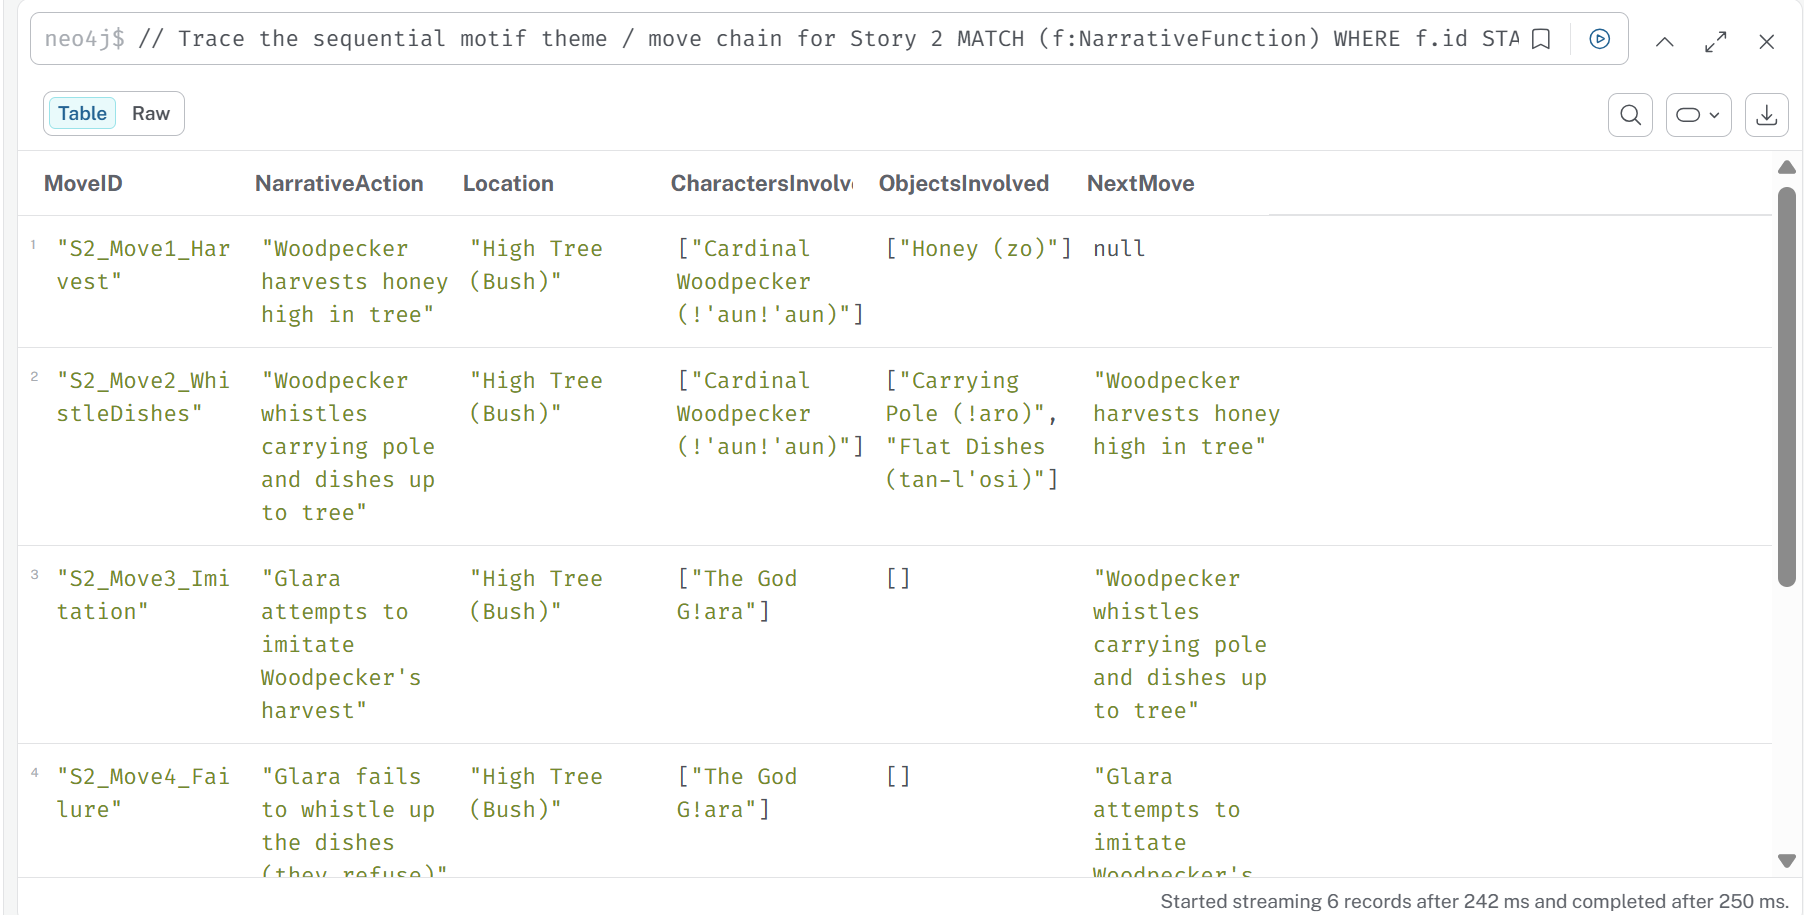
\includegraphics[width=\textwidth,trim=10 10 10 10,clip]{figures/kg-move-chain-story2.png}
% \caption{Cypher query tracing the sequential motifeme/move chain for the canonical ``Honey and the Flies'' reference story (Story 2: Woodpecker and Glara). \texttt{context\_builder.py} returns each move's \texttt{NarrativeAction}, \texttt{Location}, \texttt{CharactersInvolved}, \texttt{ObjectsInvolved}, and \texttt{NextMove} link, giving the Generator Agent an ordered structural chain rather than an unordered text excerpt.}
% \label{fig:kg-move-chain}
% \end{figure}

% \subsection{LangGraph Multi-Agent Execution Pipeline}
% The pipeline executes three nodes sequentially; this paper centers on \textbf{Agent 1 (Generator)}, which carries the core contribution, while Agents 2--3 are summarized here for pipeline completeness.

% \begin{figure}[h]
% \centering
% \begin{tikzpicture}[
%     box/.style={rectangle, draw, rounded corners, minimum width=2.8cm, minimum height=0.8cm, align=center, fill=gray!8, font=\footnotesize},
%     term/.style={rectangle, draw, rounded corners, minimum width=1.8cm, minimum height=0.7cm, align=center, font=\footnotesize},
%     dec/.style={diamond, draw, align=center, fill=gray!8, font=\footnotesize, inner sep=2pt},
%     arr/.style={-{Latex[length=2.2mm]}, thick}
% ]
% \node[term] (start) at (0,6) {start};
% \node[dec] (router) at (0,4.8) {input\_story\\provided?};
% \node[box] (echo) at (-2.6,3.2) {echo\_input\_story};
% \node[box] (gen) at (2.6,3.2) {Agent 1: Generator};
% \node[box] (cls) at (0,1.8) {Agent 2: Classifier};
% \node[box] (grd) at (0,0.6) {Agent 3: Grader};
% \node[term] (end) at (0,-0.6) {end};

% \draw[arr] (start) -- (router);
% \draw[arr] (router) -| node[pos=0.3, above, font=\tiny] {yes} (echo);
% \draw[arr] (router) -| node[pos=0.3, above, font=\tiny] {no} (gen);
% \draw[arr] (echo) |- (cls);
% \draw[arr] (gen) |- (cls);
% \draw[arr] (cls) -- (grd);
% \draw[arr] (grd) -- (end);
% \end{tikzpicture}
% \caption{LangGraph execution pipeline. A story supplied for classification-only mode bypasses generation via \texttt{echo\_input\_story}; otherwise the Generator Agent synthesizes a new narrative. Both paths converge at the Classifier and Grader nodes.}
% \label{fig:pipeline}
% \end{figure}

% \begin{enumerate}
%     \item \textbf{Agent 1 (Generator)}: Receives Neo4j subgraphs, RAG folktale excerpts, and vocabulary constraints from \texttt{ju\_dictionary.xls}. Synthesizes a structured narrative adhering to spatial dynamics (Camp $\leftrightarrow$ Bush) and Dundes motifemes.
%     \item \textbf{Agent 2 (Classifier)}: Parses generated prose using Pydantic structured output (\texttt{ClassificationOutput}), identifying present Dundes motifemes and functional plot moves.
%     \item \textbf{Agent 3 (Evaluator/Grader)}: Evaluates narrative quality along two dimensions:
%     \begin{equation}
%         \text{Score}_{\text{Cultural}} = \frac{\text{Egalitarianism} + \text{FoodSharing} + \text{Kinship}}{3}
%     \end{equation}
%     \textit{Critical Penalty}: If an unpunished resource hoarding move appears, $\text{Score}_{\text{Cultural}}$ drops to $0$.
% \end{enumerate}

% \subsection{Sample Generated Narrative}
% As a qualitative complement to the benchmark in Section~\ref{sec:results}, Figure~\ref{fig:generated_story} shows a \texttt{jnang}-generated narrative for the trickster/waterhole theme, and Figure~\ref{fig:evaluation} shows the corresponding Grader Agent evaluation report for that story.

% \begin{figure}[h]
% \centering
% 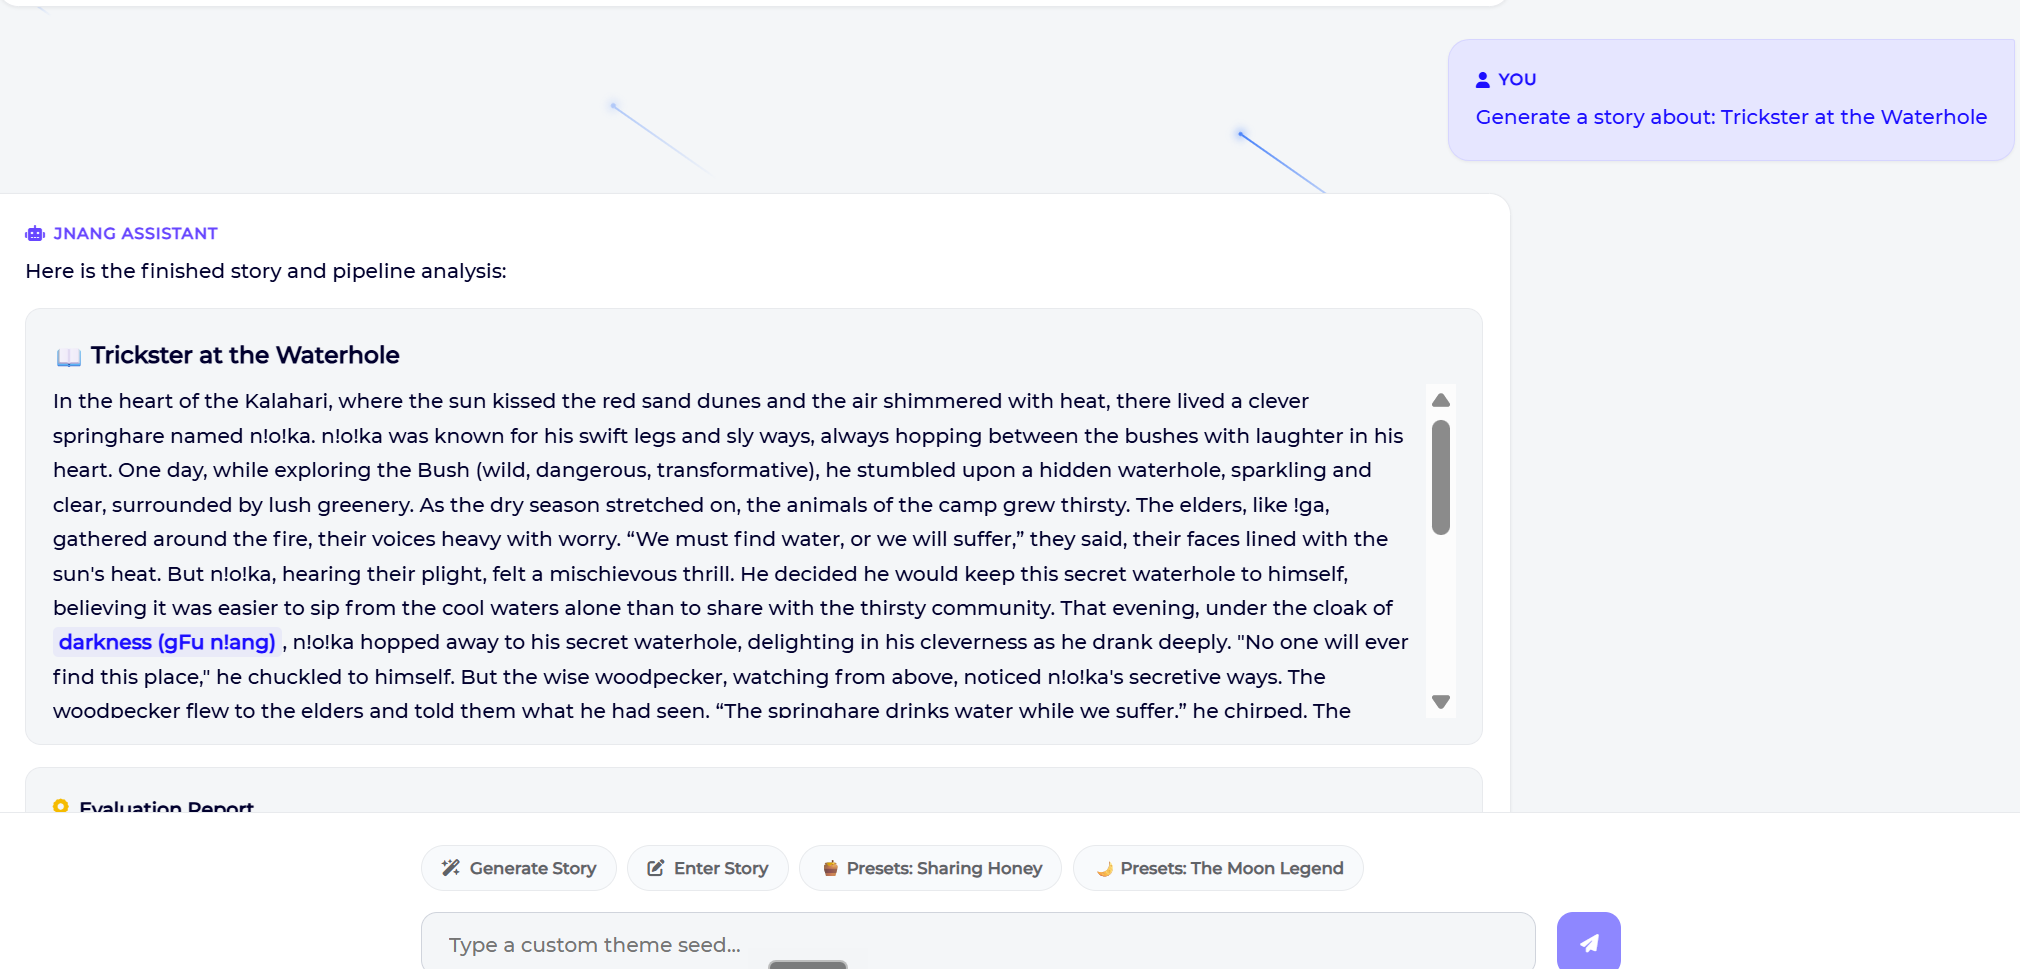
\includegraphics[width=0.9\textwidth]{story generated.png}
% \caption{Generated story based on trickster and waterhole themes.}
% \label{fig:generated_story}
% \end{figure}

% \begin{figure}[h]
% \centering
% 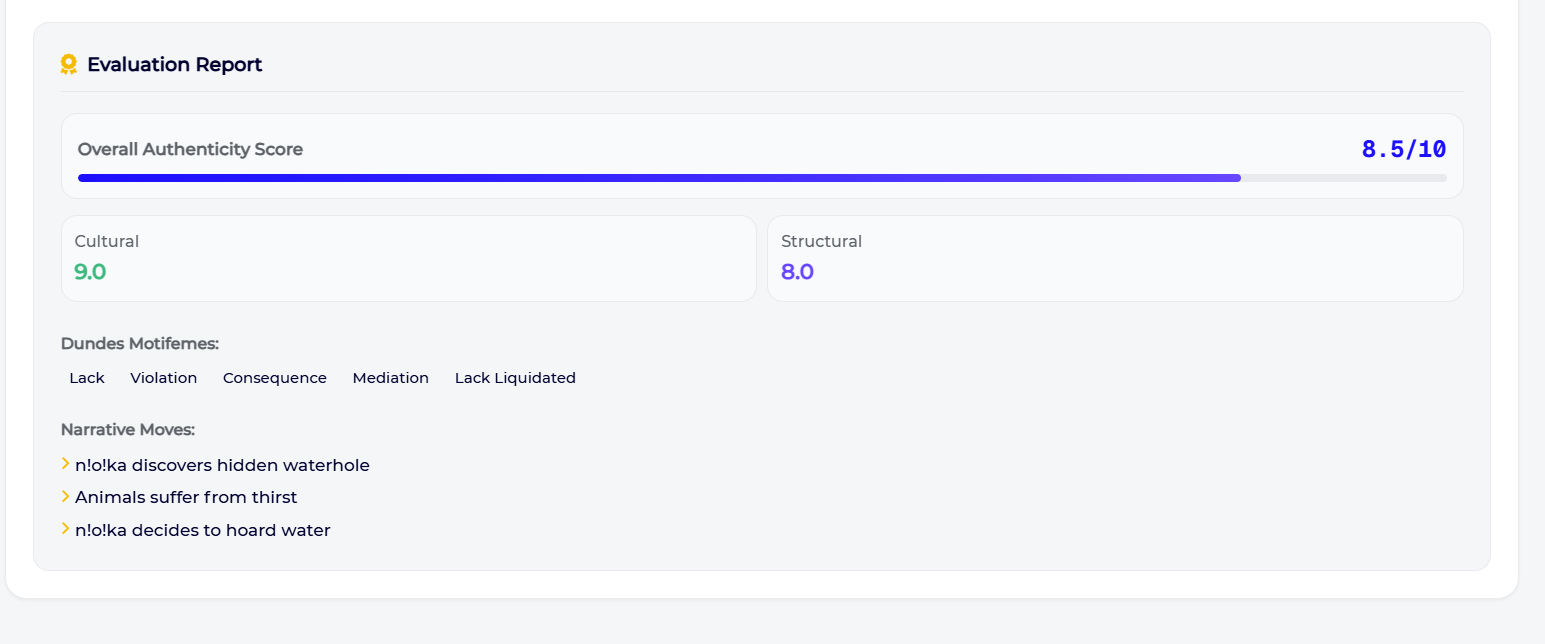
\includegraphics[width=0.9\textwidth]{grader evaluation report.png}
% \caption{Evaluation report by the Grader Agent for the story in Figure~\ref{fig:generated_story}.}
% \label{fig:evaluation}
% \end{figure}

% \section{Machine Translation \& Cultural Adaptation Framework}\label{sec:mt}

% Standard MT models lose cultural semantics when translating Western stories into indigenous languages. \texttt{jnang} provides a pre-translation adaptation layer:

% \begin{enumerate}
%     \item \textbf{Pre-Translation Oicotype Substitution}: Maps source narrative elements to local \juhoansi{} oicotypes (for example, replacing a king's decree with an elder's campfire taboo).
%     \item \textbf{Ontology-Constrained Decoding}: Hard-constrains vocabulary generation through graph relationships to enforce Khoisan click orthography ($!$, $/$, $\neq$, $//$) and exact kinship terms.
%     % \item \textbf{Automated Cultural Quality Estimation}: Uses the Grader Agent as a quality filter, rejecting translated outputs that violate communal sharing rules.
% \end{enumerate}

\subsection{System Architecture}\label{sec:architecture}

The \texttt{jnang} architecture consists of three main layers: the Semantic Ontology Layer, the Knowledge Graph Layer, and the LangGraph Multi-Agent Pipeline.

% \begin{figure}[h]
% \centering
% \begin{tikzpicture}[
% node distance=1.1cm,
% layer/.style={rectangle, draw, rounded corners, minimum width=8cm, minimum height=1.1cm, align=center, fill=gray!8},
% arr/.style={-{Latex[length=2.5mm]}, thick}
% ]
% \node[layer] (ont) {Semantic Ontology Layer\\\texttt{folktales\_ontology.ttl} (RDF/OWL)};
% \node[layer, below=of ont] (kg) {Knowledge Graph Layer\\Neo4j + \texttt{context\_builder.py}};
% \node[layer, below=of kg] (agents) {LangGraph Multi-Agent Pipeline\\Generator $\rightarrow$ Classifier $\rightarrow$ Grader};
% \draw[arr] (ont) -- (kg) node[midway, right, font=\footnotesize] {\texttt{import\_rdf.py}};
% \draw[arr] (kg) -- (agents) node[midway, right, font=\footnotesize] {Cypher subgraph retrieval};
% \end{tikzpicture}
% \caption{Three-layer \texttt{jnang} architecture. The RDF/OWL ontology is ingested into a Neo4j knowledge graph, which provides theme-matched subgraphs to the multi-agent pipeline during generation.}
% \label{fig:architecture}
% \end{figure}
\begin{figure}[h]
\centering
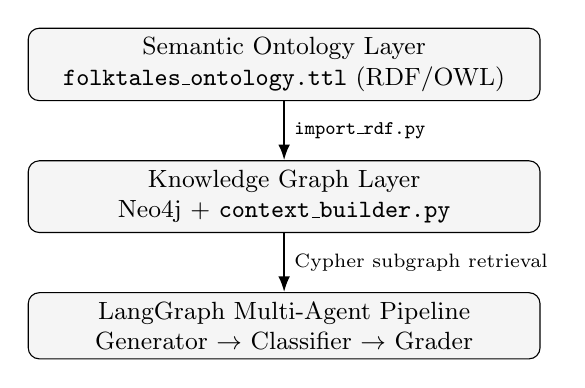
\begin{tikzpicture}[
node distance=0.75cm,
layer/.style={
    rectangle,
    draw,
    rounded corners,
    minimum width=6.5cm,
    minimum height=0.8cm,
    align=center,
    fill=gray!8,
    font=\small
},
arr/.style={-{Latex[length=2mm]}, thick}
]
\node[layer] (ont) {Semantic Ontology Layer\\\texttt{folktales\_ontology.ttl} (RDF/OWL)};
\node[layer, below=of ont] (kg) {Knowledge Graph Layer\\Neo4j + \texttt{context\_builder.py}};
\node[layer, below=of kg] (agents) {LangGraph Multi-Agent Pipeline\\Generator $\rightarrow$ Classifier $\rightarrow$ Grader};

\draw[arr] (ont) -- (kg) node[midway, right, font=\scriptsize] {\texttt{import\_rdf.py}};
\draw[arr] (kg) -- (agents) node[midway, right, font=\scriptsize] {Cypher subgraph retrieval};
\end{tikzpicture}
\caption{Three-layer \texttt{jnang} architecture. The RDF/OWL ontology is ingested into a Neo4j knowledge graph, which provides theme-matched subgraphs to the multi-agent pipeline during generation.}
\label{fig:architecture}
\end{figure}

\subsection{Corpus \& Structural Decomposition}

The source material is \textit{\juhoansi{} Folktales: Transcriptions and English Translations} \cite{biesele2009folktales}, a community-authored literacy primer containing 14 transcribed \juhoansi{} folktales with interlinear \juhoansi{}-English translations. A companion lexicon (\texttt{ju\_dictionary.xls}) contains 4{,}737 entries mapping \juhoansi{} terms to English meanings and parts of speech. This lexicon is used to constrain vocabulary generation and check orthographic accuracy.

Four of the 14 stories --- \textit{The Moon Dies and Lives Again}, \textit{The Honey and the Flies}, \textit{A Woman First Found Fire}, and \textit{The Elephant First Found Water} --- were formally represented in the seed RDF knowledge graph. An LLM was first used to propose narrative segments based on Dundes motifemes, Proppian functions, character roles, and Camp/Bush spatial locations. These annotations were then reviewed and corrected against the source transcriptions before being encoded as RDF see figure \ref{fig:architecture}. The remaining ten stories are used as unstructured RAG sources, providing additional lexical and thematic information without explicit structural annotations.


\subsection{RDF Narrative Ontology \& Neo4j Knowledge Graph}
\medskip

The narrative ontology is defined in RDF Turtle using OWL classes for characters, narrative functions, magical agents, and Proppian roles.

\begin{comment}
\begin{lstlisting}[language=TeX]
propp:Character a owl:Class .
propp:NarrativeFunction a owl:Class .
propp:MagicalAgent rdfs:subClassOf propp:Object .
propp:ProppianRole a owl:Class .
\end{lstlisting}
\end{comment}

The RDF data are imported into Neo4j using \texttt{import\_rdf.py}, creating relationships such as \texttt{:PERFORMS\_FUNCTION}, \texttt{:HAS\_ROLE}, \texttt{:LACKS}, and \texttt{:FOLLOWS}. During generation, \texttt{context\_builder.py} uses Cypher queries to retrieve subgraphs relevant to the selected narrative  see figure \ref{fig:kg-graph} and \ref{fig:kg-move-chain}. This provides the Generator Agent with both narrative content and its structural relationships.

\begin{figure}[H]
\centering
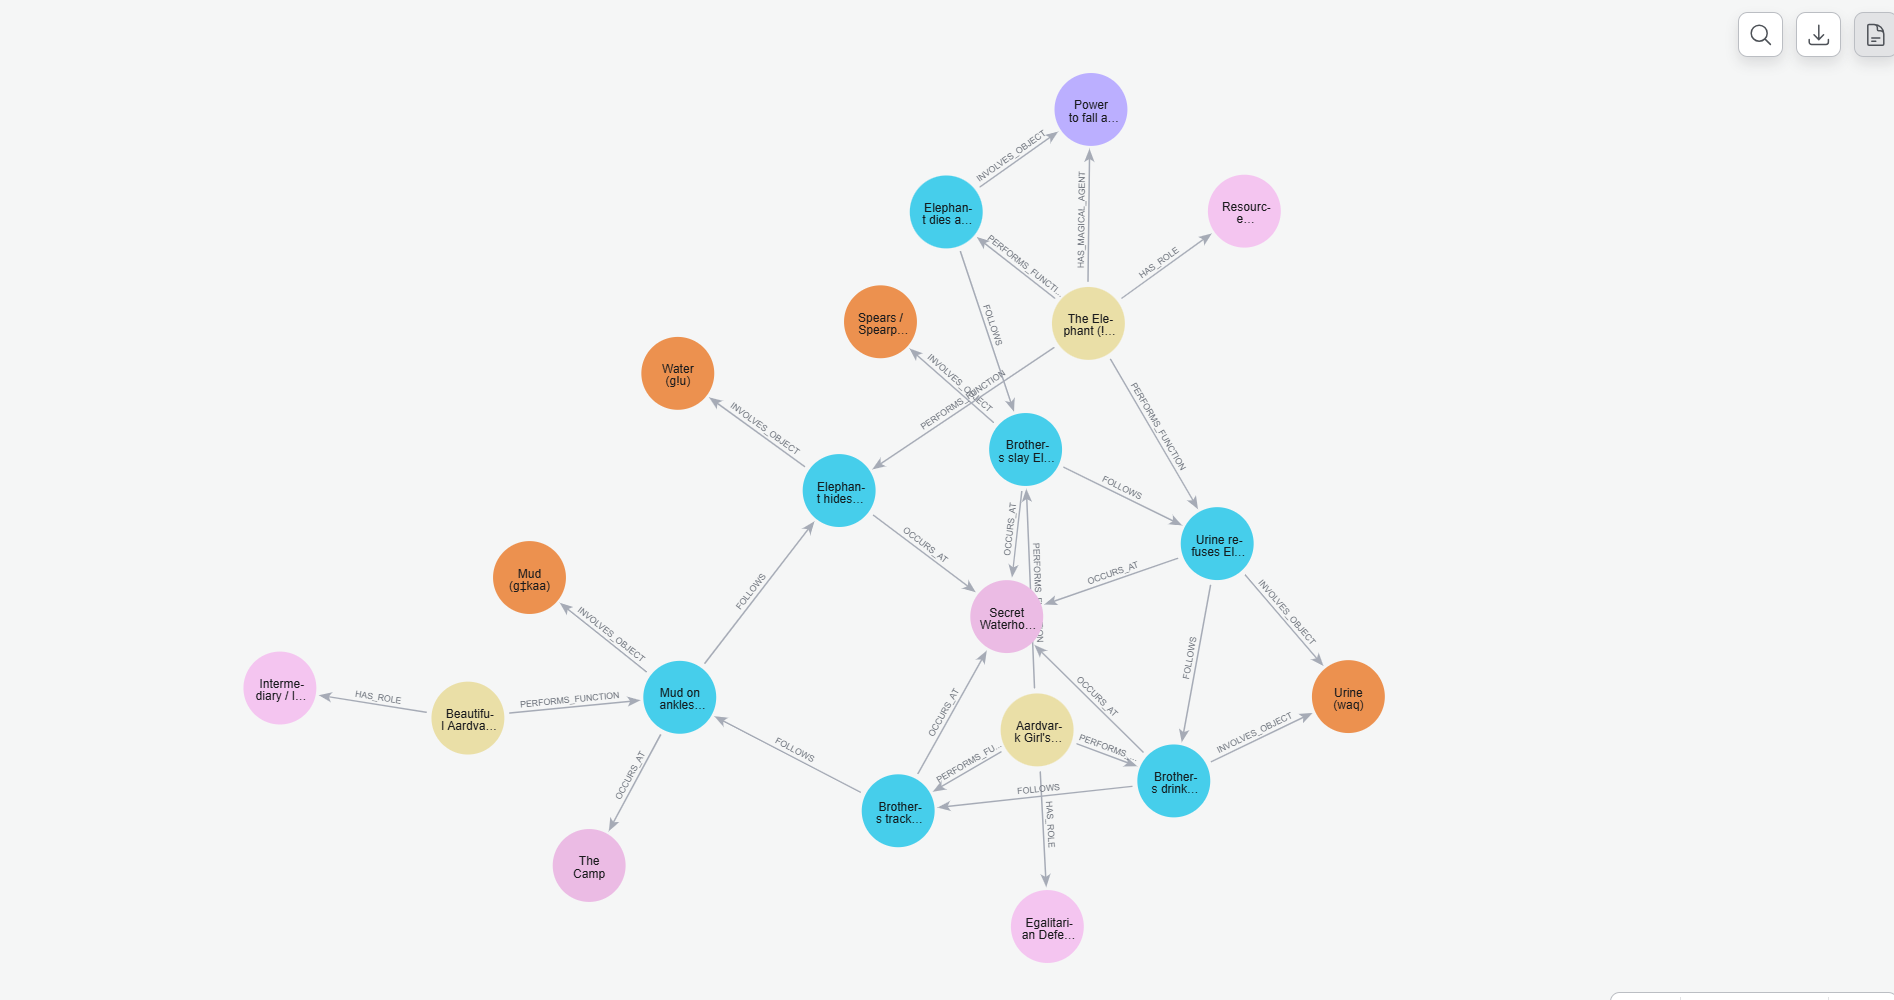
\includegraphics[width=\textwidth,trim=10 10 10 10,clip]{figures/kg-2hop-query.png}
\caption{Neo4j 2-hop neighborhood query around a story's narrative functions. The graph connects characters, narrative functions, objects, roles, and locations through typed relationships for the \textit{Elephant} story.}
\label{fig:kg-graph}
\end{figure}

\begin{figure}[H]
\centering
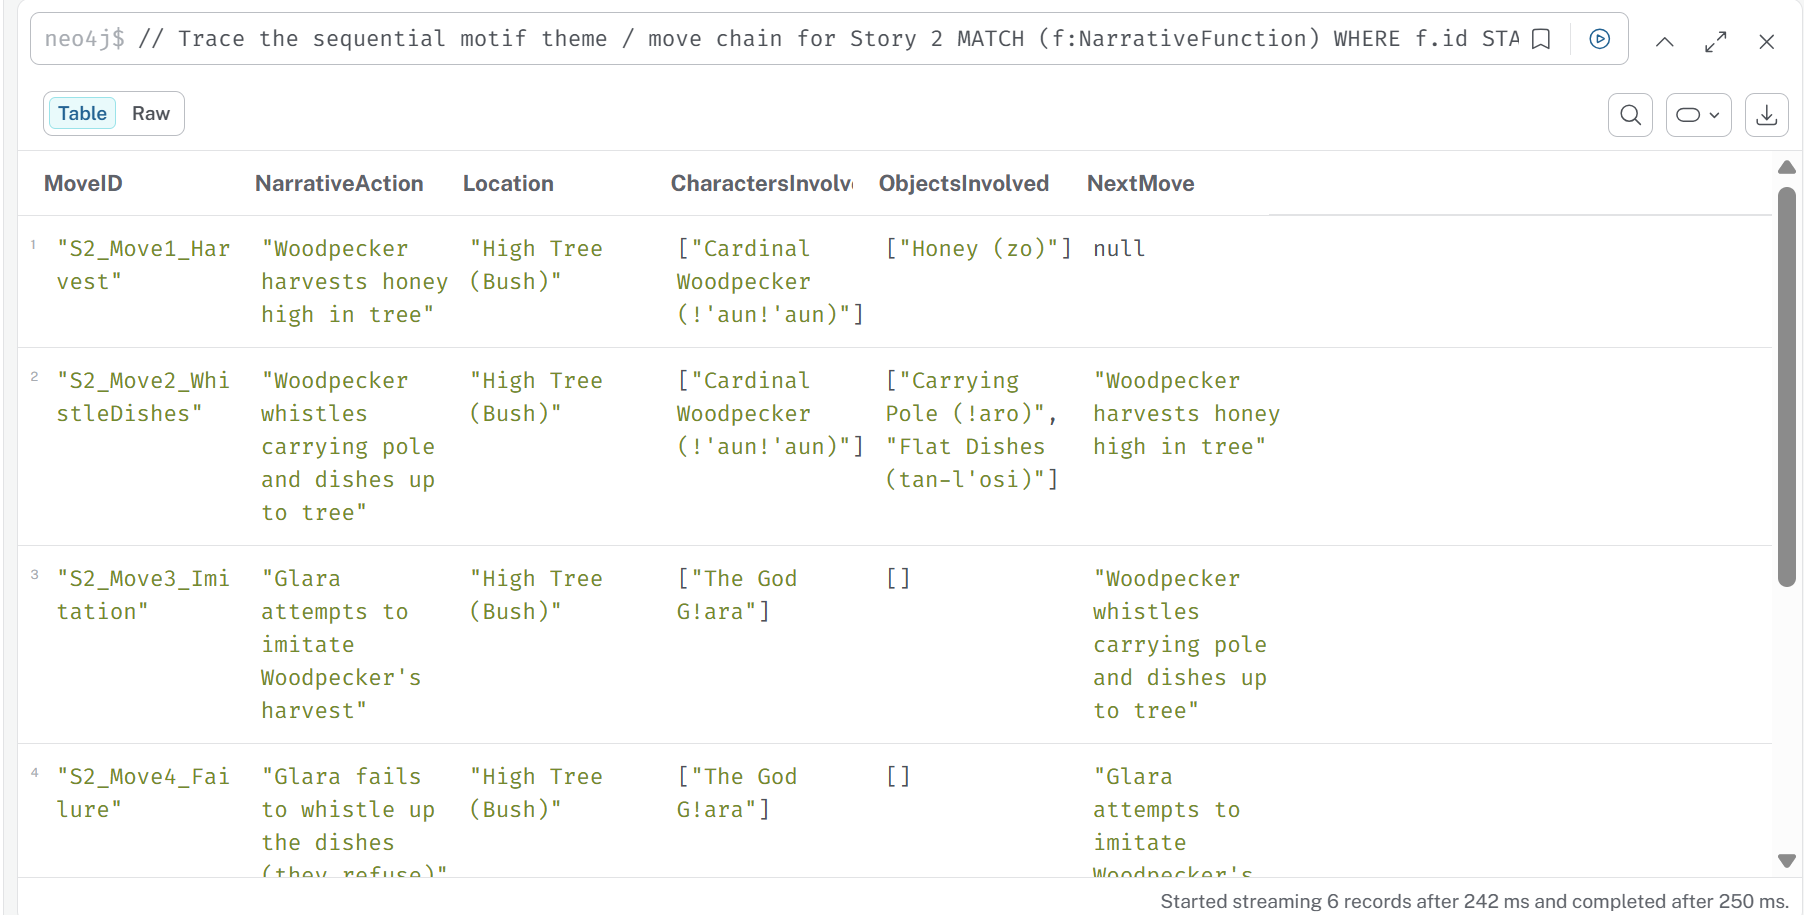
\includegraphics[width=0.8\textwidth,trim=10 10 10 10,clip]{figures/kg-move-chain-story2.png}
\caption{Cypher query tracing the sequential motifeme and narrative-move chain for the \textit{Honey and the Flies} story. The retrieved structure provides an ordered sequence of actions, locations, characters, and objects rather than an unordered text excerpt.}
\label{fig:kg-move-chain}
\end{figure}

\subsection{LangGraph Multi-Agent Execution Pipeline}

The system uses three sequential agents. The Generator performs the main narrative generation, while the Classifier and Grader provide structural analysis and evaluation see figure \ref{fig:pipeline}.

% \begin{figure}[H]
% \centering
% \begin{tikzpicture}[
% box/.style={rectangle, draw, rounded corners, minimum width=2.8cm, minimum height=0.8cm, align=center, fill=gray!8, font=\footnotesize},
% term/.style={rectangle, draw, rounded corners, minimum width=1.8cm, minimum height=0.7cm, align=center, font=\footnotesize},
% dec/.style={diamond, draw, align=center, fill=gray!8, font=\footnotesize, inner sep=2pt},
% arr/.style={-{Latex[length=2.2mm]}, thick}
% ]
% \node[term] (start) at (0,6.8) {start};
% \node[dec] (router) at (0,4.8) {input\_story\\provided?};
% \node[box] (echo) at (-2.6,3.2) {echo\_input\_story};
% \node[box] (gen) at (2.6,3.2) {Agent 1: Generator};
% \node[box] (cls) at (0,1.8) {Agent 2: Classifier};
% \node[box] (grd) at (0,0.6) {Agent 3: Grader};
% \node[term] (end) at (0,-0.6) {end};
% \draw[arr] (start) -- (router);
% \draw[arr] (router) -| node[pos=0.3, above, font=\tiny] {yes} (echo);
% \draw[arr] (router) -| node[pos=0.3, above, font=\tiny] {no} (gen);
% \draw[arr] (echo) |- (cls);
% \draw[arr] (gen) |- (cls);
% \draw[arr] (cls) -- (grd);
% \draw[arr] (grd) -- (end);
% \end{tikzpicture}
% \caption{LangGraph execution pipeline. Stories supplied for classification bypass generation, while new narratives are first produced by the Generator. Both paths then pass through the Classifier and Grader.}
% \label{fig:pipeline}
% \end{figure}

\begin{figure}[H]
\centering
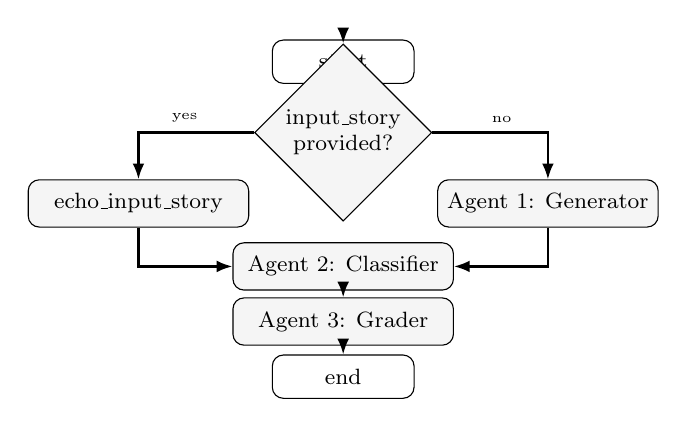
\begin{tikzpicture}[
box/.style={
    rectangle, draw, rounded corners,
    minimum width=2.8cm,
    minimum height=0.6cm,
    align=center,
    fill=gray!8,
    font=\footnotesize
},
term/.style={
    rectangle, draw, rounded corners,
    minimum width=1.8cm,
    minimum height=0.55cm,
    align=center,
    font=\footnotesize
},
dec/.style={
    diamond, draw,
    align=center,
    fill=gray!8,
    font=\footnotesize,
    inner sep=1.5pt
},
arr/.style={-{Latex[length=2mm]}, thick}
]

\node[term] (start) at (0,3.6) {start};
\node[dec] (router) at (0,2.7) {input\_story\\provided?};
\node[box] (echo) at (-2.6,1.8) {echo\_input\_story};
\node[box] (gen) at (2.6,1.8) {Agent 1: Generator};
\node[box] (cls) at (0,1.0) {Agent 2: Classifier};
\node[box] (grd) at (0,0.3) {Agent 3: Grader};
\node[term] (end) at (0,-0.4) {end};

\draw[arr] (start) -- (router);
\draw[arr] (router) -| node[pos=0.3, above, font=\tiny] {yes} (echo);
\draw[arr] (router) -| node[pos=0.3, above, font=\tiny] {no} (gen);
\draw[arr] (echo) |- (cls);
\draw[arr] (gen) |- (cls);
\draw[arr] (cls) -- (grd);
\draw[arr] (grd) -- (end);

\end{tikzpicture}
\caption{LangGraph execution pipeline. Stories supplied for classification bypass generation, while new narratives are first produced by the Generator. Both paths then pass through the Classifier and Grader.}
\label{fig:pipeline}
\end{figure}

\begin{enumerate}
\item \textbf{Generator Agent}: Receives Neo4j subgraphs, RAG folktale excerpts, and vocabulary constraints from \texttt{ju\_dictionary.xls}. It generates narratives guided by Camp/Bush spatial dynamics and Dundes motifemes (see Section~\ref{sec:results}).

\item \textbf{Classifier Agent}: Uses structured output through \texttt{ClassificationOutput} to identify Dundes motifemes and narrative-function moves present in the generated story (see figure \ref{fig:pipeline}).

\item \textbf{Grader Agent}: Evaluates narrative quality based on cultural authenticity, including egalitarianism, food sharing, and kinship. Stories containing unpunished resource hoarding receive a cultural-authenticity score of zero.
\end{enumerate}

%\subsection{Sample Generated Narrative}

%Figure~\ref{fig:generated_story} presents an example narrative generated for the trickster and waterhole themes. Figure~\ref{fig:evaluation} shows the corresponding evaluation produced by the Grader Agent.

% \begin{figure}[h]
% \centering
% 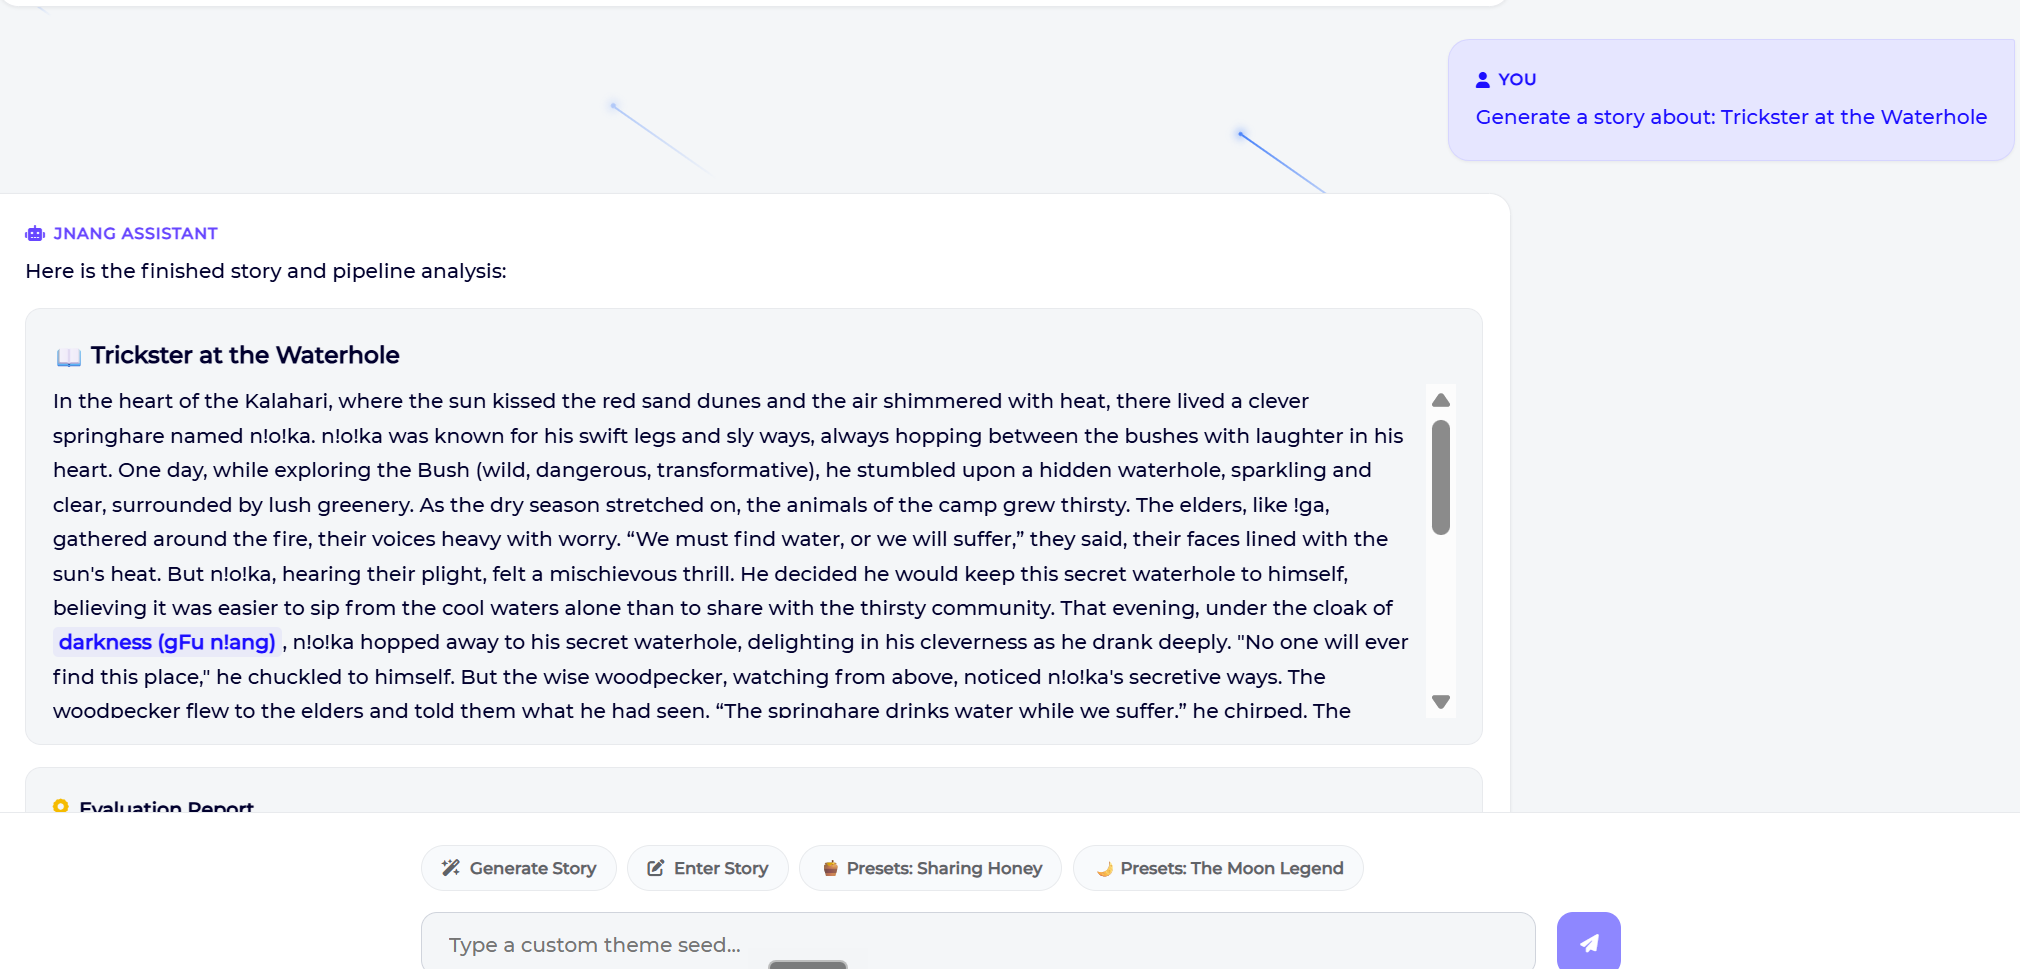
\includegraphics[width=0.9\textwidth]{story generated.png}
% \caption{Generated story based on trickster and waterhole themes.}
% \label{fig:generated_story}
% \end{figure}

% \begin{figure}[h]
% \centering
% 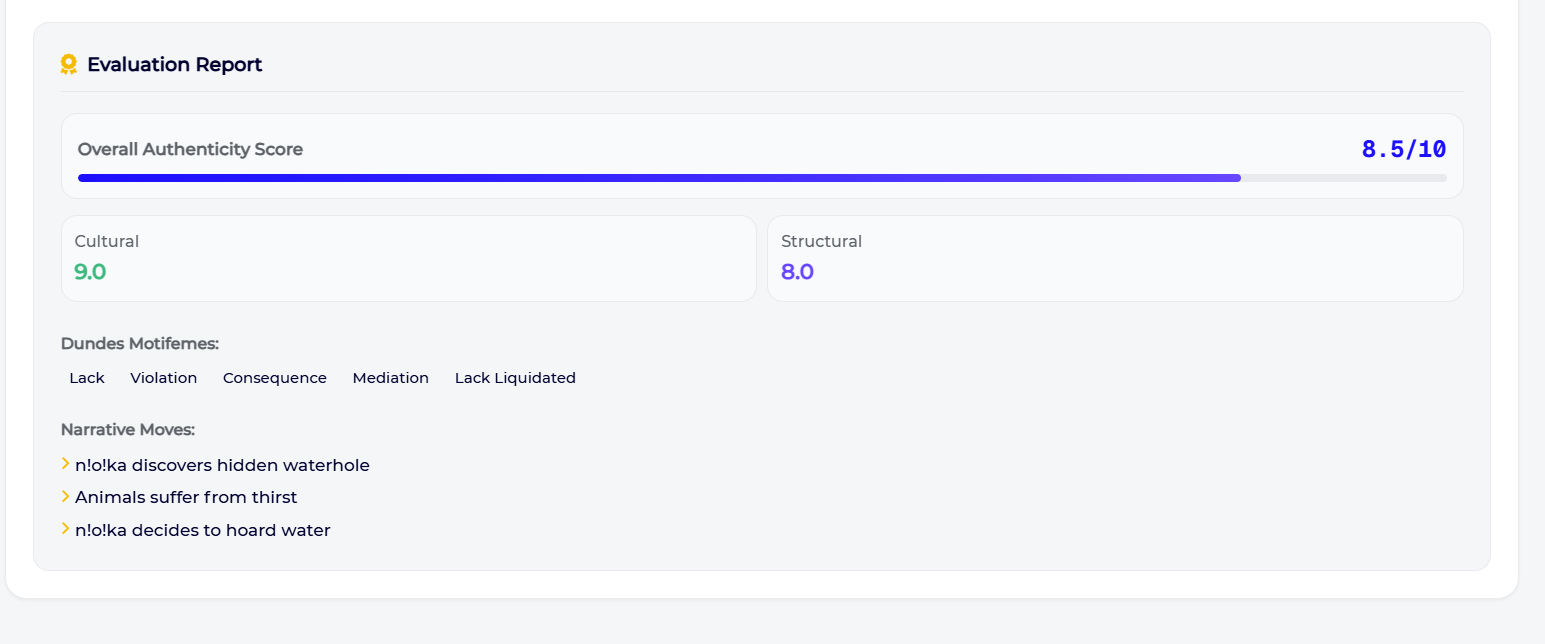
\includegraphics[width=0.9\textwidth]{grader evaluation report.png}
% \caption{Evaluation report produced by the Grader Agent for the generated story.}
% \label{fig:evaluation}
% \end{figure}

% \section{Machine Translation \& Cultural Adaptation Framework}\label{sec:mt}

% The framework can also support cultural adaptation before machine translation by incorporating local narrative structures and vocabulary. Two mechanisms are proposed:

% \begin{enumerate}
% \item \textbf{Pre-Translation Oicotype Substitution}: Replaces culturally inappropriate narrative elements with corresponding \juhoansi{} elements, such as replacing a king's decree with an elder's campfire taboo.

% \item \textbf{Ontology-Constrained Decoding}: Uses the knowledge graph and reference vocabulary to guide the generation of \juhoansi{} terms and maintain appropriate click-consonant orthography ($!$, $/$, $\neq$, $//$).
% \end{enumerate}




\section{Results \& Evaluation}\label{sec:results}

 The system was benchmarked \texttt{jnang} against a naive baseline,  the same \texttt{gpt-4o-mini} model prompted for a \juhoansi{} folktale with no ontology, knowledge graph, RAG, or dictionary grounding across 8 pre-registered themes: the 5 preset narrative themes (sharing honey, the Moon's immortality message, a trickster hiding a waterhole, the origin of fire, and the Elephant holding back water) and 3 held-out stories from the source corpus (Ostrich and the Tortoise, Springhare Dances, Ducks and People) absent from both the RDF ontology and the RAG pool, testing generalization rather than memorization. Each of the resulting 16 narratives (one per theme per arm; $N=16$, no repeats  a pilot-scale, indicative comparison rather than a powered study) was scored twice: once by the pipeline's own in-pipeline grader (\texttt{gpt-4o-mini}, the same model family as the Generator, given the Classifier's motifeme analysis as context) and once by an independent, blind judge (Gemini 2.5 Flash, given only the raw story text, with no knowledge of which arm produced it or any prior structural analysis). Two deterministic, non-LLM checks supplement both graders: a European-trope keyword scanner and a click-consonant vocabulary verifier cross-checked against the reference lexicon (\texttt{ju\_dictionary.xls}).
% here you could put a few sample sentences of the story
% \begin{table}[h]
% \caption{Arm-level means across all 8 themes ($N=8$ per arm), by grader.}\label{tab:results}
% \begin{tabular}{@{}lcccc@{}}
% \toprule
%  & \multicolumn{2}{c}{In-Pipeline Grader} & \multicolumn{2}{c}{Independent Judge} \\
% Metric & Baseline & \texttt{jnang} & Baseline & \texttt{jnang} \\
% \midrule
% Cultural Authenticity (0--10) & 4.83 & \textbf{7.42} & 2.15 & \textbf{6.36} \\
% Motifeme Coverage (0--10) & 9.00 & \textbf{9.38} & 9.00 & \textbf{9.44} \\
% No Unpunished Hoarding Rate & 62\% & 62\% & 38\% & \textbf{88\%} \\
% \bottomrule
% \end{tabular}
% \end{table}

\begin{table}[h]
\caption{Arm-level means across all 8 themes ($N=8$ per arm), by grader.}\label{tab:results}
\begin{tabular}{@{}lcccc@{}}
\toprule
 & \multicolumn{2}{c}{In-Pipeline Grader} & \multicolumn{2}{c}{Independent Judge} \\
Metric & Baseline & \texttt{jnang} & Baseline & \texttt{jnang} \\
\midrule
Cultural Authenticity (0--10) & 4.83 & \textbf{7.42} & 2.15 & \textbf{6.36} \\
Motifeme Coverage (0--10) & 9.00 & \textbf{9.38} & 9.00 & \textbf{9.44} \\
No Unpunished Hoarding Rate & 62\% & 62\% & 38\% & \textbf{88\%} \\
\bottomrule
\end{tabular}
\end{table}




\noindent \textbf{Cultural authenticity.}

\noindent  Under the independent judge, \texttt{jnang} scored higher than the baseline on cultural authenticity in all 8 themes ($k = 8$ of $n = 8$ positive differences). A one-sided sign test yields $p = 0.5^{8} \approx 0.004$, rejecting the null hypothesis of equal performance. Because the test relies on sign counts rather than score magnitudes, it is sensitive to even a single reversal: if one theme flipped direction, $k = 7$ of $n = 8$ would give $p \approx 0.035$, still below $\alpha = 0.05$ but substantially weaker. The deterministic trope scanner provides independent, non-LLM support for this result: the baseline produced European terms such as ``king'' and ``gold'' in 2 of 8 stories, while \texttt{jnang} produced none.

\medskip

\noindent \textbf{Sample output.}

\noindent The following excerpt is from the \texttt{jnang} narrative for the trickster and
waterhole theme:

\begin{quote}
\small
``The elders, including his wise grandmother, $!ga$, gathered around the campfire each evening
\ldots{} But Tjua, instead of sharing this precious secret with the thirsty community, decided to
keep it all for himself. \ldots{} Just as he leaned down to drink, the water began to swirl and
shimmer, transforming into a great $g//awasi$ spirit \ldots{} \emph{You have kept the life of the
community from them! You must return what you have stolen!} \ldots{} He led them to the hidden
waterhole \ldots{} and as they drank, they laughed and danced, sharing the life-giving water.''
\end{quote}

\noindent The Classifier labelled this chain Lack $\rightarrow$ Interdiction $\rightarrow$
Violation $\rightarrow$ Consequence $\rightarrow$ Mediation $\rightarrow$ Lack Liquidated, and the
independent judge recovered the same positions from the text alone. The excerpt also exposes a
recurring flaw: in 4 of the 8 \texttt{jnang} narratives the Generator names motifeme labels in the
prose rather than only enacting them, an artefact of the structural prompt that a production
version would need to suppress.

\medskip

\noindent \textbf{Self-grading bias.}

\noindent  The two graders showed substantial disagreement. Their overall grades matched in only 5 of 16 cases (31\%), and their cultural-authenticity scores differed by an average of 1.87 points. The in-pipeline grader also rated the baseline much more favorably than the independent judge (4.83 vs. 2.15), while the scores for \texttt{jnang} were more similar (7.42 vs. 6.36). This suggests that using a grader from the same model family as the Generator may overestimate performance, supporting the use of an independent judge.

\medskip

\noindent \textbf{Hoarding-rule interpretation.}

\noindent  Both graders apply the same hard rule: each is instructed that rewarded or unpunished resource hoarding sets the corresponding sub-score to zero, and both derive an overall grade of \textit{Fails} when that occurs. The instruments differ in model family and in the information they receive, not in this criterion. The in-pipeline Grader Agent sees the Classifier's motifeme analysis alongside the story; the independent judge sees only the raw narrative text. The gap in Table~\ref{tab:results} (No Unpunished Hoarding Rate: 88\% for \texttt{jnang} vs. 38\% for the baseline under the independent judge) is therefore a like-for-like comparison under an identical rule, applied by a model outside the Generator's family.

\medskip

\noindent \textbf{Generalization.}

\noindent  Three themes absent from both the RDF ontology and RAG pool tested out-of-distribution generalization. Table~\ref{tab:generalization} reports these separately from the 5 preset themes.

\begin{table}[h]
\caption{Cultural authenticity by theme subset (independent judge).}\label{tab:generalization}
\begin{tabular}{@{}lccc@{}}
\toprule
Theme Subset & Baseline & \texttt{jnang} & $\Delta$ \\
\midrule
\multicolumn{4}{@{}l}{\textit{Preset themes ($n=5$)}} \\
\quad Sharing Honey & 7.17 & 9.50 & +2.33 \\
\quad Moon's Immortality & 0.70 & 8.00 & +7.30 \\
\quad Trickster Waterhole & 0.67 & 8.00 & +7.33 \\
\quad Origin of Fire & 3.33 & 8.20 & +4.87 \\
\quad Elephant Holds Water & 0.00 & 5.33 & +5.33 \\
\quad \textit{Preset mean} & \textit{2.37} & \textit{7.81} & \textit{+5.43} \\
\midrule
\multicolumn{4}{@{}l}{\textit{Held-out themes ($n=3$)}} \\
\quad Ostrich and the Tortoise & 1.00 & 4.00 & +3.00 \\
\quad Springhare Dances & 0.33 & 1.67 & +1.34 \\
\quad Ducks and People & 4.00 & 6.20 & +2.20 \\
\quad \textit{Held-out mean} & \textit{1.78} & \textit{3.96} & \textit{+2.18} \\
\bottomrule
\end{tabular}
\end{table}

\noindent  \texttt{jnang} outperformed the baseline on all 3 held-out themes, but the mean gain ($+2.18$) was less than half the preset-theme gain ($+5.43$). This pattern is consistent with the architecture: the Generator Agent's structural context comes from Cypher-retrieved subgraphs, and held-out themes have no graph-encoded motifeme chains to retrieve. The result suggests that the ontology provides genuine structural grounding rather than memorized retrieval, but also that generalization weakens when graph coverage is incomplete.

\medskip

\noindent  \textbf{Orthographic precision.}

\noindent Orthographic accuracy remains a limitation that undercuts the orthographic-precision objective stated in Section~\ref{sec:intro}. Of the 11 click-consonant glossed terms produced across all 8 \texttt{jnang} stories, only 4 (36\%) could be verified against the reference lexicon (\texttt{ju\_dictionary.xls}). The unverified terms fall into two categories: hardcoded vocabulary in the Generator Agent's system prompt that does not match the reference lexicon's entry format (e.g. kinship and spirit terms), and terms generated by the LLM for concepts outside the lexicon's 4{,}737-entry coverage. The baseline produced zero glossed \juhoansi{} terms, making direct comparison impossible. A story can therefore pass every cultural and structural check while still containing invented or incorrect \juhoansi{} words. Future work should audit and align the hardcoded vocabulary with the reference lexicon and expand lexicon coverage rather than relying on LLM-generated orthography.




\section{Conclusion}\label{sec:conclusion}

\texttt{jnang} combines indigenous \juhoansi{} oral traditions with agentic narrative generation. By pairing a Neo4j knowledge graph encoding Dundes' motifemes and Camp/Bush spatial structure with a multi-agent LangGraph pipeline, the system produces narratives that are structurally constrained by \juhoansi{} cultural mechanics rather than by Indo-European quest arcs. In a pilot comparison against a naive \texttt{gpt-4o-mini} baseline, \texttt{jnang} scored higher on cultural authenticity across all 8 themes under independent judging (sign test, $p \approx 0.004$) and produced zero European tropes.

%\textbf{Community evaluation gap.} 
Cultural authenticity has only been judged by LLMs and a keyword scanner. No \juhoansi{} community members, elders, or cultural experts participated in evaluating the generated stories. The pilot results demonstrate computational consistency rather than cultural validity. %A cultural validation with \juhoansi{} community members has been planned to substantiate cultural authenticity.

The evaluation was small ($N=16$ narratives, no repeated samples per condition), and results should be viewed as indicative rather than conclusive. The two LLM-based graders agreed on overall grade in only 31\% of cases, and the in-pipeline grader systematically overestimated baseline quality. The current knowledge graph covers only four of the 14 stories in the source corpus, and only 36\% of generated click-consonant terms could be verified against the reference lexicon.

Future work will expand the knowledge graph to the remaining corpus stories, conduct cultural validation with \juhoansi{} speakers and cultural experts, audit the Generator Agent's hardcoded vocabulary against the reference lexicon, and explore the framework's applicability to other indigenous oral traditions.


% \section*{Declarations}
% \begin{itemize}
% \item \textbf{Funding}: Supported by the Department of Software Engineering, Namibia University of Science and Technology (NUST).
% \item \textbf{Conflict of Interest}: The authors declare no competing interests.
% \item \textbf{Data Availability}: All ontology triples (\texttt{.ttl}), Neo4j import scripts, and agent code are available in the project repository.
% \end{itemize}


\begingroup
\small
\medskip
\bibliography{sn-bibliography}
\endgroup

\end{document}
